\documentclass[11pt, letterpaper, fleqn]{article}
\usepackage[super,numbers,sort&compress,square]{natbib}
\usepackage{fancyhdr}
\usepackage{enumitem}
\usepackage{amsmath}
\usepackage{amssymb}
\usepackage{bm}
\usepackage{graphicx}
\newcommand{\R}{\mathbb{R}}
% \DeclareMathOperator*{\argmax}{argmax}




\usepackage[dvipsnames]{xcolor}

\usepackage{fancyvrb}

% redefine \VerbatimInput
\RecustomVerbatimCommand{\VerbatimInput}{VerbatimInput}%
{fontsize=\footnotesize,
 %
 frame=lines,  % top and bottom rule only
 framesep=2em, % separation between frame and text
 rulecolor=\color{Gray},
 %
 label=\fbox{\color{Black}topicwords.csv},
 labelposition=topline,
 %
 commandchars=\|\(\), % escape character and argument delimiters for
                      % commands within the verbatim
 commentchar=*        % comment character
}




\topmargin=-0.45in
\evensidemargin=0in
\oddsidemargin=0in
\textwidth=6.5in
\textheight=9.0in
\headsep=0.25in

\setlength\parindent{0pt}

\pagestyle{fancy}
\lhead{Saurabh Mathur}
\rhead{CSCI B555 (Prof. Roni Khardon): Programming Project 4}
%\rhead{\firstxmark}
%\lfoot{\lastxmark}
\cfoot{\thepage}

\title{\textbf{Programming Project 4 for CSCI B555}}
\author{Saurabh Mathur}
\date{\today}

%\graphicspath{{figures/}}

\begin{document}

\maketitle

\section*{Task 1}

\subsection*{Code}
The solution code for Task 1 resides in task1.py and can be run as \\

\$ python3 task1.py


\subsection*{Questions}
Do the topics make sense for the dataset ?

Yes, the topics do seem to make sense. For example 1,2,3 and 5 clearly seem to talk about automobiles and 4 and 7 clearly talk about space.

\VerbatimInput{topicwords.csv}

\begin{figure}
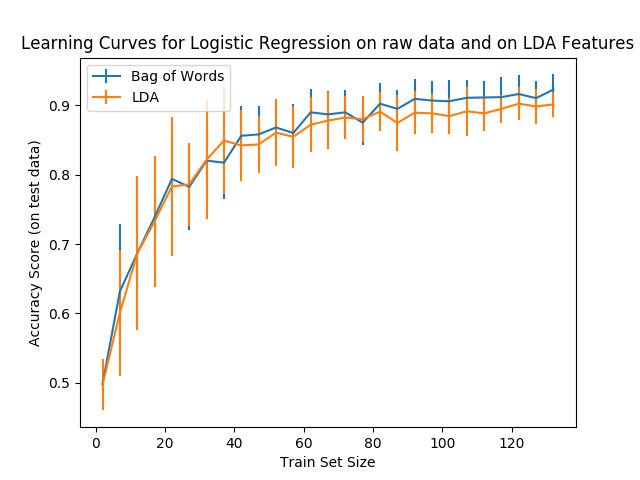
\includegraphics[width=\textwidth]{Figure_1.png}
\caption{Test set accuracy as a function of increasing train set size}
\label{fig:1a}
\end{figure}


\section*{Task 2}

\subsection*{Code}
The solution code for Task 2 resides in task1.py and can be run as \\

\$ python3 task2.py


\subsection*{Discussion of results}
In the bag of words model each word is a feature and so it has close to 400 features. On the other hand, for the LDA based logistic regression model there are only 20 features, one feature for each topic. So, the size of the LDA based model is about 20 times smaller than the bag of words model.\\

Figure \ref{fig:1a} depicts the learning curve for bag of words (raw data) based and LDA based logistic regression. For less training data, the LDA model seems to perform at par and even better than the bag of words model. However, as more data is available the bag of words model starts performing better. The difference in performance is small and does not seem to grow with further increase in size of training data. 



\end{document}